%%=============================================================================
%% Fase 2: Technische analyse en experimenten
%%=============================================================================
\chapter{Technische Analyse en Experimenten}
\label{ch:fase2}
%%In deze fase was het doel om de lijst van gewenste functionele en niet-functionele requirements aan te vullen en deze te structureren naargelang hun prioriteit. Onder andere de keuze van de programmeertaal, eventuele libraries en andere softwaretools die gebruikt konden en zouden worden voor het maken en opzetten van de proof of concept werden hier gemaakt. De keuze van de programmeertaal werd bereikt door het opstellen van kleine prototypes in elke kandidaat-programmeertaal. Deze kregen werden dan getimed en daarnaast werden ook andere voor- en nadelen van elk bekeken om zo tot de beste optie te komen.

Net zoals bij alle software, was het ook hier van belang om eerst grondig onderzoek te doen naar wat er effectief nodig was en naar welke technologieën er best gebruikt konden worden.
Deze fase was van groot belang voor het verdere verloop van het project. Het was de bedoeling om een duidelijk beeld te krijgen van wat er nodig was en hoe dit het best kon worden aangepakt. Een duidelijk overzicht van de functionele en niet-functionele requirements was hierbij van groot belang. 

Als eerste werd er onderzocht wat een linter nu eigenlijk was en hoe deze werkte. Daarnaast werd er ook gekeken naar de verschillende soorten linters die er bestonden en naar de programmeertalen waarin deze gemaakt waren. Zodra duidelijk was wat er verwacht werd, werd er een lijst opgesteld van de gewenste functionele en niet-functionele requirements. Deze werden dan gestructureerd naargelang hun prioriteit zodat er bepaald kon worden wat er al dan niet tot de MVP zou behoren.

Met deze lijst kon er dan gekeken worden naar de keuze van de programmeertaal die gebruikt kon en zou worden voor het maken en opzetten van de proof of concept. De keuze van de programmeertaal werd bereikt door het opstellen van kleine prototypes in elke kandidaat-programmeertaal. Deze kregen werden dan getimed en daarnaast werden ook andere voor- en nadelen van elk bekeken om zo tot de beste optie te komen.

Uit de lijst van functionaliteiten werden er twee gekozen die als eerste uitgewerkt zouden worden om zo een eerste versie van de linter te bekomen. Deze functionaliteiten waren: het detecteren van duplicaten en de detectie om te zien of alle required fields wel aanwezig waren.

% ---
% \section{Linters onder de loep}
% \label{sec:linters-onder-de-loep}

% Gezien er tot op heden slechts één linter beschikbaar was voor BibLaTeX en deze niet optimaal leek te zijn, werd er besloten om ook eens te kijken naar andere linters die er bestonden. Zo kon er inspiratie opgedaan worden voor de proof of concept die gemaakt zou worden. Linters die werden bekeken zijn: Ruff, Pytype, Flake8, DirtyRat, bibl en nog enkele andere. De linters diende net zoals het proof of concept open-source en gratis te gebruiken zijn.

%  \subsection{BibLaTeX linter}
% \label{sec:biblatex-linter}
% Zoals reeds vermeld, was er tot op heden nog geen \emph{optimale} BibLaTeX linter beschikbaar. 

% Onderzoek wees uit dat de linter van Pez Cuckow\footnote{\url{https://github.com/Pezmc/BibLatex-Linter}} de enige linter was die specifiek voor BibLaTeX gemaakt was. Hoewel de linter een web-ui heeft, werd er tijdens dit onderzoek niet in geslaagd om een bestand succesvol te laten valideren. Een poging om een bestand te valideren, leidde tot volgende de foutmelding die te zien is op afbeelding \ref{fig:biblatex-linter-error}.

% \begin{figure}[ht]
%     \centering
%     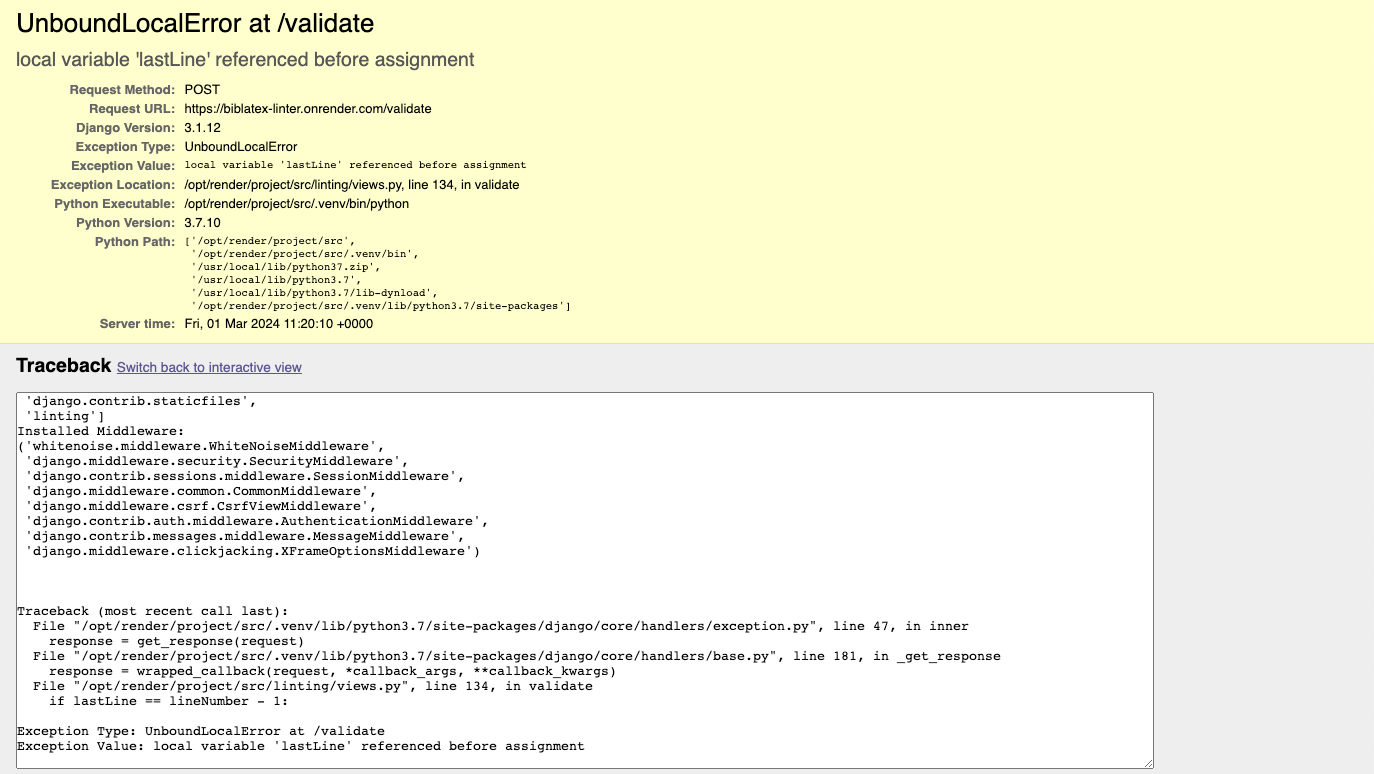
\includegraphics[width=0.7\textwidth]{./files/Pezmc-LinterError_cropped.png}
%     \caption[Foutmelding BibLaTeX-linter]{Lintingerror bij het valideren van een BibLaTeX bestand.}
%     \label{fig:biblatex-linter-error}
% \end{figure}

% Daarnaast leek de aanpak van de geschreven code ook niet optimaal te zijn op vlak van leesbaarheid en uitbreidbaarheid. Gezien dit echter wel criteria zijn waar de proof of concept aan moest voldoen, werd er besloten om deze linter niet verder te onderzoeken. Er werd wel gekeken naar de functionaliteiten die deze linter aanbood en andere zaken die handig leken om over te nemen in de eigen implementatie.


% \subsection{Ruff versus de concurrentie}
% \label{subsec:ruff}
% Ruff\footnote{\url{https://astral.sh/ruff}} is een Python linter geschreven in Rust. Dat is ook direct waar Ruff zich onderscheid van de concurrent Python linters die gewoon in Python geschreven zijn. Rust is een programmeertaal die bekend staat om zeer snel en veilig te zijn. Dit zou dus duidelijk een goede keuze kunnen zijn voor een linter. Daarnaast is Rust ook veel lichter om te draaien op hardware dan Python, gezien Python een interpretatieve taal is en Rust een gecompileerde taal. 
% Dit zou dus ook een goede keuze kunnen zijn voor een linter die in een CI-pipeline gebruikt zou worden. Ook is er slechts één versie van Rust waar steeds op verdergewerkt wordt, hierdoor wensen de developers van de Rust taal ook dat de code die in Rust geschreven wordt, steeds blijft werken. Of het nu over vijf jaar is, of over tien jaar, wat vandaag gecompileerd kan worden, zal ook binnen tien jaar nog steeds gecompileerd kunnen worden. 

% Ruff zou op bepaalde taken tien tot wel honderd keer sneller kunnen zijn! Dit wekte direct al interesse op om de Rust taal eens op de proef te stellen om te zien of dit ook effectief zo was. 


% ---
\section{Functionele en Niet-Functionele Requirements}
Nadat de volledige reeks linters was geanalyseerd, kon een lijst van zowel functionele als niet-functionele vereisten worden opgesteld. Dankzij de promotor van deze thesis werd dat proces versneld. Een informatieve lijst werd verstrekt, waarin onder andere een opsomming van de gewenste regels stond. Aangezien de promotor uitgebreide technische kennis van het onderwerp heeft en beschouwd kan worden als de \emph{klant} bij de ontwikkeling van deze tool, werd gefocust op de uitwerking van de specifieke regels volgens zijn wensen.\newline

Een overzicht van de \textbf{functionele requirements} kan in tabel \ref{tab:functional_requirements} worden bezichtigd. Merk op dat deze lijst slechts een richtlijn is voor tijdens de effectieve uitwerking.\newline

Wat de \textbf{niet-functionele} requirements betreft:
\begin{itemize}
    \item Er wordt gewenst dat de linter gebruikt kan worden vanuit de \textbf{CLI} zodat deze in pipelines gebruikt kan worden.
    \item De linter dient \textbf{vlot} te werken, zodat de tool strict als handig beschouwd kan worden en zeker niet als iets storend.
    \item De linter dient \textbf{uitbreidbaar} te zijn eens deze proef-periode is afgelopen. Er wordt duidelijke, gestructureerde en gedocumenteerde code verwacht.
    \item Er wordt verwacht dat het \textbf{eenvoudig} te gebruiken is, begrijp hieronder dat het beschikbaar zal zijn via een pip-installatie gelijk andere Python modules.
\end{itemize}

\begin{table}[ht]
    \centering
    \begin{tabular}{p{2.5cm} p{13cm}}
        \toprule
        \textbf{Prioriteit} & \textbf{Requirement Beschrijving} \\
        \midrule
        \textbf{Musts} & 
          - Elk item moet een sleutel hebben. \\
        & - Elke BibLaTeX-sleutel moet uniek zijn. \\
        & - Alle vereiste velden moeten aanwezig en niet leeg zijn. \\
        & - Auteurnamen moeten in het juiste formaat zijn. \\
        & - Data moeten in het formaat `YYYY-MM-DD` zijn. \\
        & - Speciale tekens te vervangen door hun LaTeX-commando's. \\
        & - Paginabereiken moeten een "em-dash" gebruiken, d.w.z. `--`. \\
        & - article - Vereist: author, title, journaltitle, date. \\
        & - book - Vereist: author|editor, title, date, publisher. \\
        & - inbook - Vereist: author|editor, title, booktitle, date, publisher. \\
        & - dataset - Vereist: author|editor, title, date, url, urldate. \\
        & - manual - Vereist: author|editor, title, date. \\
        & - misc (software) - Vereist: author|editor, title, date. \\
        & - online - Vereist: author|editor, title, date, url, urldate. \\
        & - inproceedings (conference) - Vereist: author, title, booktitle, date. \\
        & - report (techreport) - Vereist: author, title, date, type, institution. \\
        & - thesis (mastersthesis, phdthesis) - Vereist: author, title, date, type, institution. \\
        \midrule
        \textbf{Shoulds} 
        & - Geef de voorkeur aan "date" boven "year" en/of "month". \\
        & - Aanbevolen velden \texttt{$(`WARN\_FIELDS`)$} moeten aanwezig en niet leeg zijn. \\
        & - article - Aanbevolen: doi, volume, number, pages. \\
        & - book - Aanbevolen: isbn. \\
        & - inbook - Aanbevolen: isbn|doi, pages. \\
        & - manual - Aanbevolen: organization|publisher, isbn|doi|url. \\
        & - inproceedings - Aanbevolen: editor, eventtitle, isbn|doi|url. \\
        & - report - Aanbevolen: doi|url. \\
        & - thesis - Aanbevolen: url. \\
        \midrule
        \textbf{Coulds} & 
          - BibLaTeX-keys moeten overeenkomen met de naam van de auteur. \\
        & - Geef de voorkeur aan originele types, niet aan aliassen. \\
        & - Verwijder tekstmarkering van URL. \\
        & - Vermijd het citeren van tertiaire bronnen. \\
        & - Citeer geen startpagina van een website. \\
        & - Geef de voorkeur aan "journaltitle" boven "journal". \\
        & - Geef de voorkeur aan "institution" boven "school". \\
        \bottomrule
    \end{tabular}
    \caption{Geprioriteerde Functionele Vereisten met behulp van de MoSCoW-methode}
    \label{tab:functional_requirements}
    \end{table}

\section{Keuze van de Programmeertaal}
\label{sec:mini-pocs}
Om de gepaste programmeertaal te vinden, werden diverse kandidaat\babelhyphen{hard}programmeertalen overwogen. De kandidaat\babelhyphen{hard}programmeertalen waren: Rust, JavaScript en Python.

Door het analyseren van reeds bestaande linters en het afgaan van een hele lijst aan programmeertalen, werd er besloten om met deze drie programmeertalen te experimenteren. Om ervoor te zorgen dat de testprogramma's niet te uitgebreid werden en zowel gelijk als eerlijk konden worden vergeleken, zouden er slechts twee functionaliteiten worden uitgewerkt. Deze twee functionaliteiten waren: detecteren van duplicaten en detecteren of alle required fields aanwezig waren. Om dit onderzoek niet nodeloos lang te maken, werd er besloten om de broncode van deze programma's niet op te nemen in dit document. De broncode is echter wel te vinden op GitHub voor zowel de kleine poc's\footnote{\url{https://github.com/MrClassicT/bibLaTeX-linter-pocs}} als voor het uiteindelijk resultaat\footnote{\url{https://github.com/MrClassicT/bibla}}.

Het test .bib bestand dat gebruik werd, zag er als volgt uit:

\inputminted[autogobble, breaklines, linenos, samepage]{bibtex} % bibtex taal wordt hier gebruikt omdat dit het dichtste aansluit bij bibLaTeX van de beschikbare opties.
{./files/test.bib} % Het test bestand van de proof of concept linters in de 3 programmeertalen.

\subsection{JavaScript}
% Een zeer gekende scripting taal dat cross-platform gebruikt kan worden. Hoewel het eerder gericht is voor het gebruik in websites of GUI gerichte scripts, is het ook mogelijk om er cli-tools mee te maken. De performantie werd onderzocht. JavaScript is ook een dynamisch typerende taal, wat in theorie voor problemen zou kunnen zorgen in sommige use-cases, al leek dit geen zorg te zijn voor deze proof of concept\autocite{Simpson2023}.

JavaScript is een programmeertaal die zeer toegankelijk en gekend is onder de meeste developers. Dit was ook de eerste programmeertaal waarin een testversie werd opgesteld, deze werd dan achteraf verteld naar zowel Python als Rust om te kijken welke van de drie talen het meest geschikt was voor deze case. 

De JavaScript versie was van een persoonlijk perspectief de beste om mee te beginnen gezien dit de meest vertrouwde taal was. Direct kan er al opgemerkt worden dat er gebruik gemaakt werd van modules, dit was noodzakelijk om de linter overzichtelijk, uitbreidbaar en onderhoudbaar te maken. Moest alles in éénzelfde bestand zitten, zou het veel te groot en onoverzichtelijk worden.

\begin{minted}[autogobble, breaklines, linenos, samepage]{javascript}
// Import submodules
const { exit } = require('process');
const { readFromFile } = require('./helper/readFromFileAsync.js');
const { checkForMissingFields } = require('./checks/missingfields.js');
const { checkForDuplicates } = require('./checks/duplicates.js');
const { entryPattern } = require('./components/regex.js');
const { toFileUrl } = require('./helper/getFileUrl.js')
\end{minted}

Als eerste wordt er een bestand ingelezen. Eens dat gebeurt is, dient er een onderscheid gemaakt te worden tussen alle verschillende bronnen binnen dit bestand. De bronnen in dit bestand, worden ook wel 'entries' genoemd. Dit werd op de volgende manier gedaan:
\begin{minted}[autogobble, breaklines, linenos, samepage]{javascript}
 // Extract all entries
 const entries = [...fileContent.matchAll(entryPattern)].map(match => ({
        type: match[1],
        citationName: match[2].trim(),
        content: match[3],
        position: match.index
    }));
\end{minted}
Op deze wijze werd niet alleen een 'entry' ontdekt, maar werd ook meteen onderscheid gemaakt tussen de bronsoort, de sleutel, de inhoud en de positie van waar deze voorkomt in het bestand. Om dit te doen, werd er gebruik gemaakt van een reguliere expressie. Met een reguliere expressie is het mogelijk om patronen binnen teksten te vinden. Gezien de structurele vorm van een .bib bestand, is het mogelijk om reguliere expressies op een eenvoudige manier te benutten om zo een krachtige analyse uit te voeren op de input.

In detail zal er niet ingegaan worden op hoe deze reguliere expressies werken, maar de twee reguliere expressies die nodig waren binnen deze mini-poc waren de volgende:
\begin{minted}[autogobble, breaklines, linenos, samepage]{javascript}
// Extract each entry from the .bib file.
const entryPattern = /@(\w+)\{([^,]+),\s*(.*?)\},\s*\}/sg;
// Extract each field from the entry.
const fieldPattern = /(\w+)\s*=\s*(?:\{(.*?)\}|(\S+))/sg;
\end{minted}

De eerste zorgt ervoor dat elke bron van elkaar onderscheden kan worden. De tweede gaat dan weer van toepassing zijn op een iets lager niveau. Daarmee kan er binnen een bron gekeken worden naar de individuele velden data die ervan bijgehouden worden, of juist om te kijken naar welke velden er missen bijvoorbeeld.

Om te kijken welke velden er missen, werd volgende methode gebruikt:

\begin{minted}[autogobble, breaklines, linenos, samepage]{javascript}
function checkForMissingFields(entry) {

    let fields = {};

    while ((fieldMatch = fieldPattern.exec(entry.content)) !== null) {
        fields[fieldMatch[1]] = fieldMatch[2] || fieldMatch[3];
    }

    let missingFields = [];
    if (entryRequirements[entry.type]) {
        entryRequirements[entry.type].required.forEach(field => {
            if (!fields[field]) {
                missingFields.push(field);
            }
        });
}

return missingFields;
}
\end{minted}
Hier wordt er een lijst gebruikt van velden die binnen de entry voor dienen te komen. Indien er gemerkt wordt dat er een bepaald veld niet in voorkomt, wordt de naam van het ontbrekende veld toegevoegd aan een lijst die teruggegeven wordt eens alles gecontroleerd is. Deze lijst wordt dan getoond aan de user.

Vóór het onderzoek naar ontbrekende velden wordt eerst gecontroleerd op eventuele duplicate entries. Ook wordt onderzocht of er mogelijk entries zijn die licht verschillen maar toch dezelfde verwijzingssleutel bevatten. Gezien het feit dat een duplicaat sleutel niet is toegestaan, wordt deze controle als eerste uitgevoerd.

\begin{minipage}{\pdfpagewidth}
Deze controle werd als volgt geïmplementeerd:

\begin{minted}[autogobble, breaklines, linenos, samepage]{javascript}
function checkForDuplicates(entries) {
    const citationNames = entries.map(entry => entry.citationName);
    const duplicates = citationNames.filter((citationName, index, self) => 
    self.indexOf(citationName) !== index 
    && self.lastIndexOf(citationName) === index
    );

    if (duplicates.length > 0) {
        const plural = duplicates.length > 1;
        console.error(`Caution: ${plural ? "" : "A "}duplicate key
        ${plural ? "s" : ""} ${duplicates} ha${plural ? "ve" : "s"} 
        been found!`);
        exit(1);
    }
}
\end{minted}
\end{minipage}
In deze controle valt op dat er een gebrek aan consistentie is in de manier waarop informatie aan de gebruiker wordt gepresenteerd. In tegenstelling tot de andere controle, waarbij dit pas achteraf gebeurde, gebeurt dit hier onmiddellijk zodra we het detecteren. Dit kan worden toegeschreven aan het feit dat dit een testversie is, ontworpen om een eerste indruk te krijgen. Bovendien zou een directe presentatie van de informatie mogelijk efficiënter kunnen zijn dan wanneer deze eerst wordt teruggestuurd naar een hoger niveau in het programma.

\subsection{Python}
\label{subsec:python}
Gezien het grote aanbod aan linters die in Python geschreven zijn en de ruime gekendheid ervan, werd er besloten om ook Python een kans te geven. Omdat de Python-kennis wat afgezwakt was, werd er beroep gedaan op de krachten van AI. De linter poc geschreven in JavaScript werd aan ChatGPT-4 gegeven en stapsgewijs werd er gevraagd om deze code om te vormen naar een werkend Python alternatief. Op enkele uren tijd werd erin geslaagd om een eerste versie werkende te krijgen. Het was zeer knap om te zien hoe goed ChatGPT met de Python syntax effectief kon omgaan. Ook de reguliere expressies die gebruikt werden, hebben op een bepaald moment in de handen van ChatGPT of zelfs github-copilot gezeten. AI-tools zijn zeer handig om complexe zaken enerzijds te verduidelijken als anderzijds erbij te assisteren om suggesties te doen van hoe een bepaald probleem aangepakt kan worden. Het potentiëel van AI was dus hier zeker merkbaar en werd ten volste benut waar mogelijk.
\pagebreak
\begin{minted}[autogobble, breaklines, linenos, samepage]{python3}
    entries = [match.groups() for match in entry_pattern.finditer(file_content)]
    formatted_entries = [{
        'type': entry[0],
        'citationName': entry[1].strip(),
        'content': entry[2],
        'position': match.start()
    } for match, entry in zip(entry_pattern.finditer(file_content), entries)]

\end{minted}

Als deze pythoncode vergeleken wordt met de javascript-code, kan er direct opgemerkt worden dat er gelijkaardige logica achter zit. Dit is uiteindelijk ook het geval want de javascript-code is simpelweg vertaald naar Python code.

De twee functionaliteiten werden op een gelijke wijze vertaald en geïmplementeerd in de kleine Python poc.

\begin{minted}[autogobble, breaklines, linenos, samepage]{python3}
def check_for_missing_fields(entry):
    fields = {}
    for match in field_pattern.finditer(entry['content']):
        key, value1, value2 = match.groups()
        fields[key] = value1 or value2

    missing_fields = []
    if entry['type'] in entry_requirements:
        for field in entry_requirements[entry['type']]['required']:
            if field not in fields:
                missing_fields.append(field)

    return missing_fields

def check_for_duplicates(entries):
    citation_names = [entry['citationName'] for entry in entries]
    duplicates = {name for name in citation_names if citation_names.count(name) > 1}
    if duplicates:
        plural = len(duplicates) > 1
        print(f'Caution: {"A duplicate key" if not plural else "Duplicate keys"} {"has" if not plural else "have"} been found: {", ".join(duplicates)}!')
        exit(1)
\end{minted}

Nadelen zijn er natuurlijk ook aan het vertalen van bestaande code naar een andere programmeertaal met behulp van AI. Zo zullen fouten die in de ene taal bestaan, hoogstwaarschijnlijk ook gewoon mee vertaald worden. Dit was bijvoorbeeld het geval wat de reguliere expressie betrefde. Bij een eerste iteratie van deze poc, werkte één van de twee controles niet. Dit bleek achteraf te komen doordat de reguliere expressie iets te gevoelig was aan de hoeveelheid witruimte die er was. Gelukkig kon deze fout relatief snel achterhaald en opgelost worden.

Ook is het interessant om te weten dat bij deze poc het programma minder modulair was. Dit kwam door een kennisbarrière waarbij niet gekend was hoe modules echt goed werken in Python. Echter was dit geen dramatisch probleem gezien het maar een kleine poc was en de zekerheid er was dat dit met wat grondiger onderzoek op een later tijdstip opgelost zou kunnen worden.

De eerste signalen dat een goede syntax-kennis niet onbelangrijk is, doken hier al op.

\subsection{Rust}
Hoewel Rust een grote kans leek te maken om de programmeertaal te worden waarin de linter geschreven zou worden, werd er dan ook vol enthousiasme aan begonnen. Snelheid is niet de enige belangrijke factor. Ook kennis is van groot belang zoals al gemerkt werd bij de Python poc. Een taal kan nog zo snel zijn, als er niemand is die er mee kan werken, dan is het nutteloos. Rust is een taal die nog niet zo lang (sinds 2015) bestaat en waar nog niet zoveel mensen mee werken, ondanks dat deze al in de top 20 meest populaire programmeertalen staat in de TIOBE Index\footnote{\url{https://www.tiobe.com/tiobe-index/}}.

Zoals eerder al enkele keren vermeld werd, was de keuze van de programmeertaal van groot belang zodat er ook na deze proef verder kon gewerkt worden aan de linter. Rust heeft daarbij de minst gunstige positie. Het was dus van groot belang om te kijken of het potentiëel in snelheid merkbaar genoeg was om de keuze te maken.

Ondanks dat er wat kennis opgedaan werd over de programmeertaal zelf, was het niet mogelijk om beide functionaliteiten werkende te krijgen binnen de Rust-poc. De kennis was simpelweg nog altijd te beperkt.
Daarom werd er besloten om de enige werkende functionaliteit te testen ten opzichte van de snelste andere poc, waarbij ook daar slechts enkel die éne controle gebruikt zou worden.

De enige functionaleit die werkend gekregen was in Rust, was de controle op duplicaten. Dit voelde toch wel als een kleine teleurstelling aan, maar vestigde nog maar eens een belang van een programmeertaal te beheersen en dat enkel AI en wat ideeën niet altijd voldoende zal zijn. Dat gaf dan ook maar direct het gevoel van jobzekerheid als programmeur.

Net zoals bij de andere twee poc's, werd er een soortgelijke werkwijze gehanteerd. Eerst worden de veschillende entries van elkaar gescheiden en vervolgens worden er de controles, of in dit geval de controle, op uitgevoerd.
\begin{minted}[autogobble, breaklines, linenos, samepage]{rust}
    let entry_pattern = &patterns::patterns::ENTRY_PATTERN;

    let entries: Vec<_> = entry_pattern
        .captures_iter(&file_content)
        .map(|cap| {
            let entry_type = cap[1].to_owned();
            let citation_name = cap[2].trim().to_owned();
            let content = cap[3].to_owned();
            let line_number = file_content[..cap.get(0).unwrap().start()].lines().count();
            (entry_type, citation_name, content, line_number)
        })
        .collect();

    checker::checker::check_for_duplicates(
        &entries
            .iter()
            .map(|(a, b, c, d)| (a.as_str(), b.as_str(), c.as_str(), *d))
            .collect::<Vec<_>>(),
        &file_path,
    );
\end{minted}

Iedereen die wat programmeerkennis heeft, kan zelf ook inzien dat deze code ver van optimaal is. Maar opnieuw, de kennisbarrière was eenmaal aanwezig en met een beperkte tijd, diende er compromis gemaakt te worden. Merk op dat er veel lussen gebeuren, lussen die hoogstwaarschijnlijk overbodig of toch zeker weg te werken zijn. Er werden veel transformaties gemaakt met de data waarbij het leek dat er van het éne type naar het andere gegaan werd om dan vervolgens terug naar het éne type te gaan. Duidelijk veel overbodigheden. Voorgaande code bevatte niet eens de volledige check op duplicaten, dat was slechts het begin-bestand waaruit de applicatie start. Hieronder volgt de effectieve controle. Merk ook daar op dat er twee lussen in de methode zitten. Hoewel het grotendeels is voor zaken op een mooie manier te tonen is, blijft het merkwaardig dat er geen efficiëntere manier gevonden kon worden. ChatGPT of Github Copilot konden hier beide niet beter mee helpen dan ze tot dit punt al gedaan hebben.

\begin{minted}[autogobble, breaklines, linenos, samepage]{rust}
    pub fn check_for_duplicates<'a>(
        entries: &[(&'a str, &'a str, &'a str, usize)],
        file_path: &str,
    ) {
        let mut duplicates: Vec<(&str, usize)> = Vec::new();
        let mut seen: Vec<&str> = Vec::new();

        for entry in entries.iter() {
            let citation_name = entry.1;
            if seen.contains(&citation_name) {
                duplicates.push((citation_name, entry.3));
            } else {
                seen.push(citation_name);
            }
        }

        for duplicate in duplicates {
            println!("All entry names should be unique.");
            let (entry_name, zerobased_line_number) = duplicate;
            let line_number = zerobased_line_number + 1;
            println!(
                "Duplicate field found in entry '{}' at line {}",
                entry_name, line_number
            );

            println!("External file path: {}:{}", file_path, line_number);
        }
    }
\end{minted}
\pagebreak  
 
\subsection{Keuze}
Na het opstellen van kleine prototypes in elke kandidaat-programmeertaal, werd er gekeken naar de voor- en nadelen van elk,en alsook naar de uitvoeringstijden. Hierbij werd er aan het begin van elk scriptje een timer gestart in de code en werd deze op het einde van de uitvoering gestopt waarna er nog een printfunctie gebeurde om het resultaat te tonen. De resultaten worden weergegeven in bijhorende tabel \ref{tabel:uitvoeringstijden}.

\begin{table}[ht]
    \centering
    \resizebox{\textwidth}{!}{
    \begin{tabular}{c|c|c|c}
        \toprule
        \textbf{JavaScript (Node)} \small{(ms)} & \textbf{Python} \small{(ms)} & \textbf{Rust} \small{(ms)} & \textbf{Notities} \\
        \midrule
        22,635 & 1.83867 & - & \multirow{3}{24em}{Eerst 3 maal Python, vervolgens 3 maal JavaScript achter elkaar.} \\
        12,008 & 1.56621 & - & \\
        13,735 & 1.57471 & - & \\
        \hline
         & & & \textbf{Commando} \\
        \hline
        
        27,095 & 1.76967 & - & {\multirow{2}{24em}{\texttt{\colorbox{bg}{node js/linter.js testData/test.bib \&\&}\break\colorbox{bg}{python3 py/linter.py testData/test.bib}}}} \\
        10,8 & 1.44262 & - &  \\
        \hline
        9,386 & 1.23654 & - & \multirow{2}{24em}{\texttt{\colorbox{bg}{python3 py/linter.py testData/test.bib}\break\colorbox{bg}{\&\& node js/linter.js testData/test.bib}}} \\
        11,311 & 1.36937 & - & \\
        \hline
        & & & \textbf{Notities} \\
        \hline
        - & 1.27763 & 9.669958 & \\
        - & 1.141 & 7.747833 & Enkel controle op duplicaten.\\
        - & 1.17904 & 8.652 &  \\
        \bottomrule
    \end{tabular}
    }
    \caption[Tabel met de uitvoeringstijden van elke poc (in milliseconden)]{De tabel met uitvoeringstijden van elke poc in vergelijking met een andere. Eerst werden JavaScript en Python met elkaar vergeleken omdat deze als eerste waren opgesteld. Achteraf werd een laatst poc in Rust opgezet. Wegens gebrek aan kennis en de tijd om deze kennis op te doen, kon er slechts één van beide controles geïmplementeerd worden. Vandaar dat bij de Rust testen genoteerd staat dat er enkel op duplicaten gecontroleerd werd. Gezien snelheid van belang was, werd JavaScript al uitgeschakeld door Python en was het dus niet nodig om deze nog eens te vergelijken met Rust.}
    \label{tabel:uitvoeringstijden}
    \end{table}

De linters werden allemaal op eenzelfde bestand gebruikt. Hierbij werd er eerst driemaal het Python commando achter elkaar uitgevoerd en daarna driemaal de JavaScript versie. Het concept van caching, opslaan van bepaalde data in snel beschikbaar geheugen, is hier zichtbaar. De eerste keer dat er iets gebeurd, duurt het langer dan de eerstvolgende keer dat het plaatsvindt.
Opmerkelijk is hier dat de JavaScript versie tot wel 12 keer \emph{trager} is dan de Python versie.

In een poging om het caching aspect te vermijden, werd het bestand nogmaals meerdere keren gecontroleerd, maar dit keer afwisselend JavaScript en Python. Eerst werd er tweemaal JavaScript als eerste uitgevoerd en vervolgens werd hetzelfde gedaan met Python als eerste. Wat extra opmerkelijk is hier, is dat JavaScript buiten gewoon lang nam in vergelijking met vorige keren. 27 milliseconden in vergelijking met de Python versie die het in minder dan 2 milliseconden kon. Hoewel het bij de tweede poging niet veel verschil maakte, kan er opnieuw gemerkt worden dat er een vorm van caching zal plaatsvinden waarbij het voorgaande resultaat nog altijd (deels) opgeslagen bleef. Hierdoor was de JavaScript linter in staat om het bestand meer dan dubbel zo snel uit te voeren. Wat wel nog altijd meer dan vijf keer trager was dan de Python versie. Python is dus een duidelijke winnaar in vergelijking met JavaScript op vlak van snelheid. Gezien Python daarnaast ook op de \emph{eerste} plaatst staat in de TIOBE Index (mei 2024), is het veilig om ervanuit te gaan dat er genoeg mensen de taal kennen om zeker te zijn dat de linter onderhoudbaar blijft nadat dit onderzoek afgelopen is.

Tot slot rest er nog Rust. Zoals eerder vermeld werd er niet in geslaagd om beide functionaliteiten werkende te krijgen. Daarom werd er besloten om enkel de controle op duplicaten uit te voeren. De snelheid van deze uitvoeringstijd, werd dan vergeleken met die van de Python versie, gezien deze de snelste van de twee was. Hoewel het internet deed geloven dat Rust mogelijk sneller zou zijn, bleek dit bij deze test verre van de waarheid te zijn. Python was ook in vergelijking met Rust sneller. Zoals eerder aangehaald, is de implementatiewijze van groot belang en mogelijks de oorzaak van deze resultaten. Echter geeft het nog altijd een realistisch beeld van de verwachten, moest er een linter in gemaakt worden. Door het gebrek aan kennis, zou de taal nooit tot het volle potentiëel benut kunnen worden en dus zou de linter nooit zo snel kunnen werken, als dat in theorie mogelijk zou moeten zijn.

Het is in principe wel nog perfect mogelijk dat Rust zich beter schaalt naar grotere bestanden toe. Het testbestand bevatte slechts één bron, maar wat als er honderden bronnen in zouden staan? Zou Python's uitvoertijd lineair vergroten of eerder exponentieel? Zou Rust sub-lineair evolueren? Deze vragen zullen binnen dit onderzoek onbeantwoord blijven. Kwestie dat er simpelweg onvoldoende tijd is om in deze scope op te nemen.\newline
Python is dus de winnaar uit dit onderzoek en zal gebruikt worden om de rest van deze proof of concept mee uit te werken.

